\documentclass[a4paper,12pt]{report}

% Pakete einbinden
\usepackage[utf8]{inputenc}
\usepackage[T1]{fontenc}
\usepackage{lipsum} % für Lorem Ipsum Beispieltext
\usepackage{graphicx} % für Bilder
\usepackage{biblatex} % für Zitate und Literaturverzeichnis
\addbibresource{bibliography.bib}

% Dokumentenbeginn
\begin{document}

% Titelblatt
\title{Titel der Diplomarbeit}
\author{Dein Name}
\date{\today}
\maketitle

% Inhaltsverzeichnis
\tableofcontents
\newpage

% Abstract
\chapter*{Abstract}
\addcontentsline{toc}{chapter}{Abstract}
\lipsum[1]

% Einleitung
\chapter{Introduction}
\lipsum[1]

% Beispielbild einfügen
\begin{figure}[h!]
    \centering
    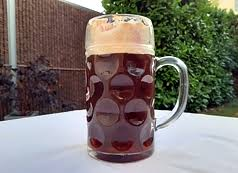
\includegraphics[width=0.5\textwidth]{bier.jpg}
    \caption{Hier ist ein Bier}
    \label{fig:beispielbild}
\end{figure}

% Hauptteil
\chapter{Main}
\lipsum[1]

% Literaturverweis-Beispiel
Hier ein Zitat aus einer Quelle \cite{author2023example}.

% Zusammenfassung
\chapter{Summary}
\lipsum[1]

% Literaturverzeichnis
\printbibliography

% Abbildungsverzeichnis
\listoffigures
\newpage

\end{document}
